
\documentclass[xetex,professionalfont]{beamer}

\usepackage{amsmath}

\usepackage{mathtools}

\usepackage{amssymb}

\usepackage{xspace}

\usepackage{booktabs}


\usepackage{fontspec}
\setmonofont[Scale=0.7]{Droid Sans Mono} %

\usepackage[caption=false]{subfig}
\captionsetup{belowskip=0pt,aboveskip=0pt}

\usepackage{csquotes}

\usepackage{copyrightbox}

\usepackage[english]{babel}


\usepackage{tikz}

\usepackage{pgfplots}

\usetikzlibrary{backgrounds,arrows,automata}

\definecolor{xblue}{RGB}{210,224,255}
\definecolor{xyellow}{RGB}{255,255,205}
\definecolor{xred}{RGB}{255,205,205}
\definecolor{xgreen}{RGB}{205,255,205}


\hypersetup{pdftitle={DLVC Lecture 10},pdfsubject={},pdfauthor={Christopher Pramerdorfer},colorlinks,urlcolor=tuwcvl_cvl_blue,linkcolor=tuwcvl_textlight,citecolor=tuwcvl_textlight}

\makeatletter\renewcommand{\CRB@setcopyrightfont}{\tiny\color{lightgray}}

\let\oldemph\emph
\renewcommand\emph[1]{\textcolor{tuwcvl_cvl_blue}{#1}}

\usefonttheme[onlymath]{serif}

\usetheme{dlvc}


\definecolor{dred}{rgb}{0.85,0,0.1}
\definecolor{dgreen}{rgb}{0,0.85,0.1}
\definecolor{dblue}{rgb}{0,0.1,0.85}


\newcommand{\ie}{\mbox{i.e.}\xspace} %
\newcommand{\eg}{\mbox{e.g.}\xspace} %

\DeclareMathOperator*{\argmin}{arg\,min}
\DeclareMathOperator*{\argmax}{arg\,max}

\newcommand{\NN}{\mathbb{N}}
\newcommand{\ZZ}{\mathbb{Z}}
\newcommand{\QQ}{\mathbb{Q}}
\newcommand{\RR}{\mathbb{R}}

\renewcommand{\vec}[1]{\ensuremath{\mathbf{#1}}}

\newcommand{\va}{\vec{a}}
\newcommand{\vb}{\vec{b}}
\newcommand{\vc}{\vec{c}}
\newcommand{\ve}{\vec{e}}
\newcommand{\vr}{\vec{r}}
\newcommand{\vs}{\vec{s}}
\newcommand{\vt}{\vec{t}}
\newcommand{\vu}{\vec{u}}
\newcommand{\vv}{\vec{v}}
\newcommand{\vw}{\vec{w}}
\newcommand{\vx}{\vec{x}}
\newcommand{\vy}{\vec{y}}
\newcommand{\vz}{\vec{z}}
\newcommand{\vo}{\vec{o}}
\newcommand{\vm}{\vec{m}}
\newcommand{\vn}{\vec{n}}

\makeatletter
\let\@@magyar@captionfix\relax
\makeatother

\newcommand{\vA}{\vec{A}}
\newcommand{\vW}{\vec{W}}
\newcommand{\vX}{\vec{X}}
\newcommand{\vY}{\vec{Y}}
\newcommand{\bth}{\boldsymbol{\theta}}
\newcommand{\cD}{\mathcal{D}}
\newcommand{\cG}{\mathcal{G}}
\newcommand{\cB}{\mathcal{B}}
\newcommand{\cF}{\mathcal{F}}

\DeclareMathOperator*{\sgn}{sgn}
\DeclareMathOperator*{\mean}{mean}
\DeclareMathOperator*{\iou}{iou}
\DeclareMathOperator*{\ap}{AP}
\DeclareMathOperator*{\map}{mAP}

\makeatletter
\def\verbatim@font{\linespread{1}\normalfont\ttfamily}
\makeatother


\title{Deep Learning for Visual Computing}
\subtitle{GANs \& Transformers}
\author{Christopher Pramerdorfer}
\institute{Computer Vision Lab, TU Wien}

\begin{document}


\begin{frame}
	\maketitle
\end{frame}


\begin{frame}
	\frametitle{Topics}

	GANs continued
	\begin{itemize}
		\item Image to image translation
		\item Other GAN variants
	\end{itemize}

	\bigskip

	Transformers
	\begin{itemize}
		\item Attention
		\item Vision transformers
	\end{itemize}

\end{frame}


\begin{frame}
	\frametitle{GANs}
	\framesubtitle{Image to Image Translation}

	Recall the following image restoration approach
	\begin{itemize}
		\item An encoder-decoder $\cG$ for image restoration
		\item A binary classiifer $\cD$ (critic) for identifying restored images
	\end{itemize}

	\smallskip

	\begin{center}
		\copyrightbox[b]
		{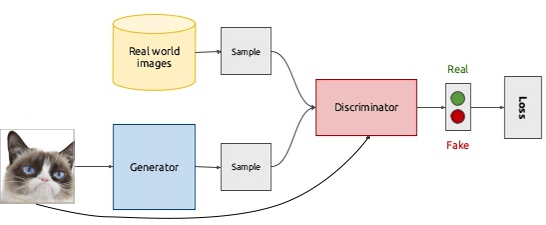
\includegraphics[width=8.5cm]{images/igan}}
		{\centering Image adapted from sigmoidal.io}
	\end{center}

\end{frame}


\begin{frame}
	\frametitle{GANs}
	\framesubtitle{Image to Image Translation}

	This is an example of \emph{image to image translation}
	\begin{itemize}
		\item $\cG$ learns to map images from domain $A$ to domain $B$
		\item In sense that $\cD$ cannot distinguish between $B$ and $\cG(A)$ %
	\end{itemize}

	\medskip

	\begin{center}
		\copyrightbox[b]
		{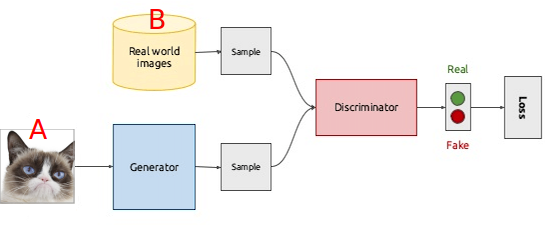
\includegraphics[width=8.5cm]{images/igan-domains}}
		{\centering Image adapted from sigmoidal.io}
	\end{center}

\end{frame}


\begin{frame}
	\frametitle{GANs}
	\framesubtitle{Image to Image Translation}

	Details depend on particular task and dataset properties
	\begin{itemize}
		\item Most importantly, are there corresponding image pairs?
	\end{itemize}

	\medskip

	\begin{center}
		\copyrightbox[b]
		{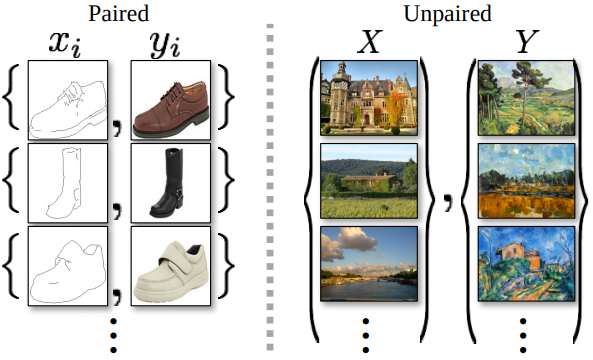
\includegraphics[width=6.5cm]{images/paired-unpaired}}
		{\centering Image from [2]. $X\mathrel{\widehat{=}}A$ and $Y\mathrel{\widehat{=}}B$.}
	\end{center}

\end{frame}


\begin{frame}
	\frametitle{GANs}
	\framesubtitle{Image to Image Translation}

	Discussed framework does not formally require image pairs

	\bigskip

	But in practice having no pairs leads to problems
	\begin{itemize}
		\item $\cG$ will have hard time fooling $\cD$ %
	\end{itemize}

	\bigskip

	Further advantages of having pairs
	\begin{itemize}
		\item Can pre-train $\cG$ to stabilize training %
		\item Can add per-pixel loss on output of $\cG$ to improve results %
	\end{itemize}

\end{frame}


\begin{frame}
	\frametitle{GANs}
	\framesubtitle{Image to Image Translation}

	Example
	\begin{itemize}
		\item Domain $A$: images of maps
		\item Domain $B$: images of areal photos
	\end{itemize}

	\medskip

	\begin{center}
		\copyrightbox[b]
		{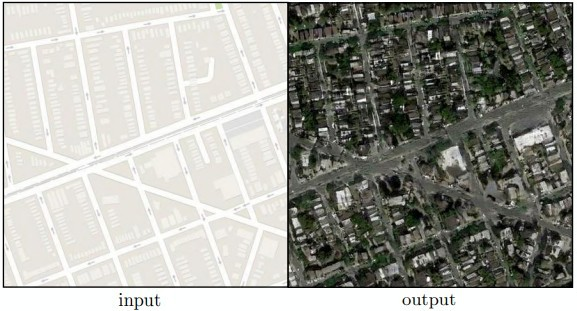
\includegraphics[width=7cm]{images/pix2pix-maps}}
		{\centering Image from [1]}
	\end{center}

\end{frame}


\begin{frame}
	\frametitle{GANs}
	\framesubtitle{Image to Image Translation}

	Example
	\begin{itemize}
		\item Domain $A$: outlines of handbags
		\item Domain $B$: images of handbags
	\end{itemize}

	\medskip

	\begin{center}
		\copyrightbox[b]
		{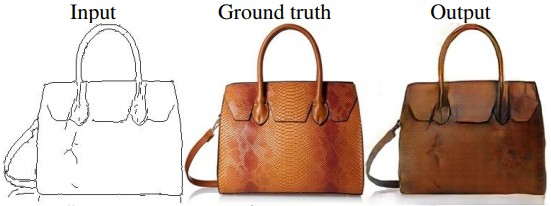
\includegraphics[width=8cm]{images/pix2pix-bags}}
		{\centering Image from [1]}
	\end{center}

\end{frame}


\begin{frame}
	\frametitle{GANs}
	\framesubtitle{Image to Image Translation}

	Example
	\begin{itemize}
		\item Domain $A$: grayscale images
		\item Domain $B$: color images
	\end{itemize}

	\medskip

	\begin{center}
		\copyrightbox[b]
		{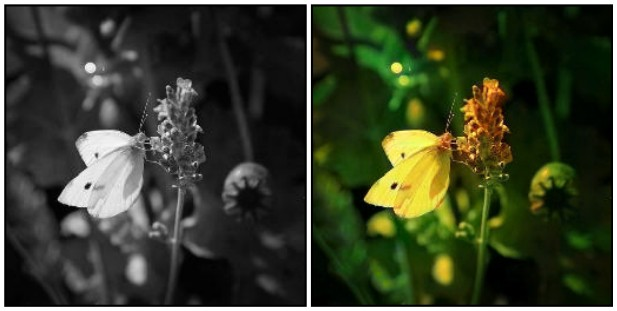
\includegraphics[width=7cm]{images/pix2pix-grayscale}}
		{\centering Image from [1]}
	\end{center}

\end{frame}


\begin{frame}
	\frametitle{GANs}
	\framesubtitle{Unpaired Image to Image Translation}

	What if image pairs are not available / possible?
	\begin{itemize}
		\item Photos to paintings, summer to winter etc.
	\end{itemize}

	\medskip

	\begin{center}
		\copyrightbox[b]
		{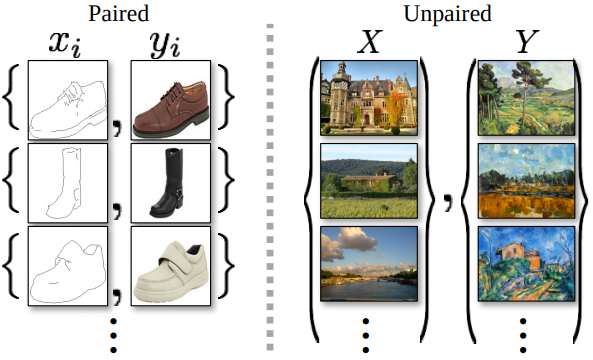
\includegraphics[width=6.5cm]{images/paired-unpaired}}
		{\centering Image from [2]. $X\mathrel{\widehat{=}}A$ and $Y\mathrel{\widehat{=}}B$.}
	\end{center}

\end{frame}


\begin{frame}
	\frametitle{GANs}
	\framesubtitle{Unpaired Image to Image Translation}

	A popular method that makes this work is \emph{CycleGAN} [2]
	\begin{itemize}
		\item Two generators $\cG:A\mapsto B$ and $\cF:B\mapsto A$
	\end{itemize}

	\bigskip

	Core idea is that we demand \emph{cycle consistency} %
	\begin{itemize}
		\item $\cF(\cG(\vx))\approx\vx$ for $\vx\in A$
		\item $\cG(\cF(\vy))\approx\vy$ for $\vy\in B$
	\end{itemize}

	\bigskip

	Generators should preserve images from target domains
	\begin{itemize}
		\item $\cG(\vy)\approx\vy$ for $\vy\in B$
		\item $\cF(\vx)\approx\vx$ for $\vx\in A$
	\end{itemize}

\end{frame}


\begin{frame}
	\frametitle{GANs}
	\framesubtitle{Unpaired Image to Image Translation}

	Four corresponding per-pixel (L1) loss functions
	\begin{itemize}
		\item For cycle-consistency: $(\vx,\cF(\cG(\vx)))$ and $(\vy,\cG(\cF(\vy)))$
		\item For identity: $(\vy,\cG(\vy))$ and $(\vx,\cF(\vx))$
	\end{itemize}

	\bigskip

	Plus two adversarial losses / discriminators $\cD_A$ and $\cD_B$
	\begin{itemize}
		\item Purpose identical to other GANs
		\item Distinguish real and fake images in domains $A$ and $B$
	\end{itemize}

	\bigskip

	Total training loss is weighted sum of all losses

\end{frame}


\begin{frame}
	\frametitle{GANs}
	\framesubtitle{Unpaired Image to Image Translation}

	\begin{center}
		\copyrightbox[b]
		{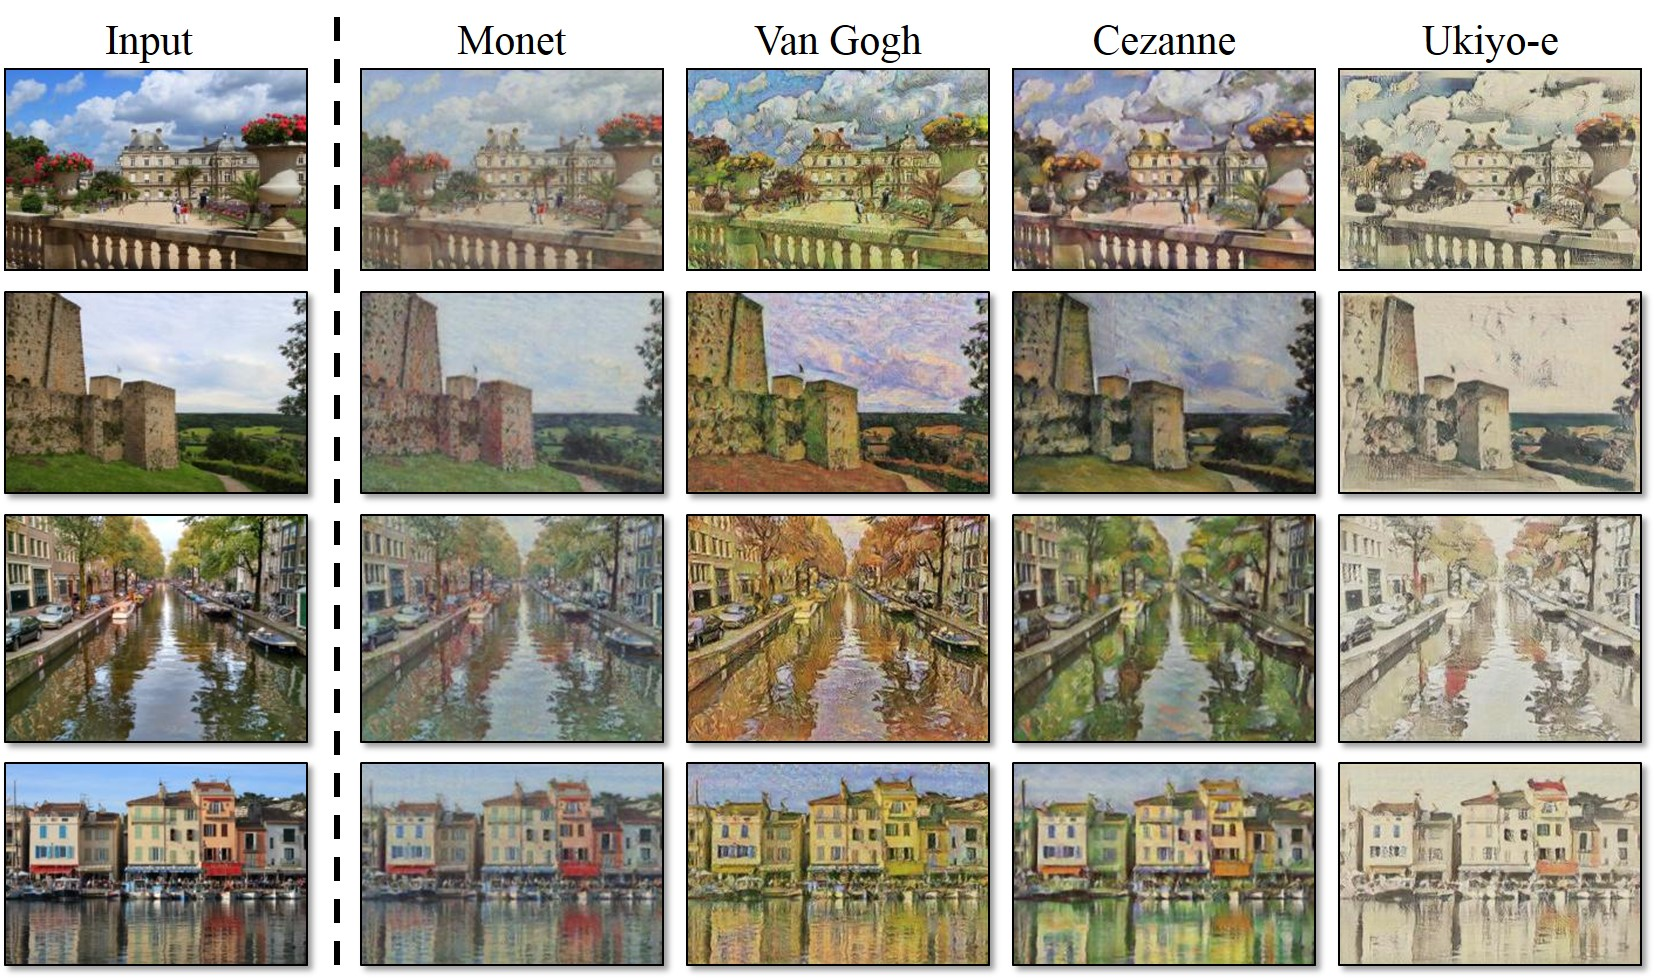
\includegraphics[width=10cm]{images/cyclegan-paintings}}
		{\centering Image from [2]}
	\end{center}

\end{frame}


\begin{frame}
	\frametitle{GANs}
	\framesubtitle{Unpaired Image to Image Translation}

	\begin{center}
		\copyrightbox[b]
		{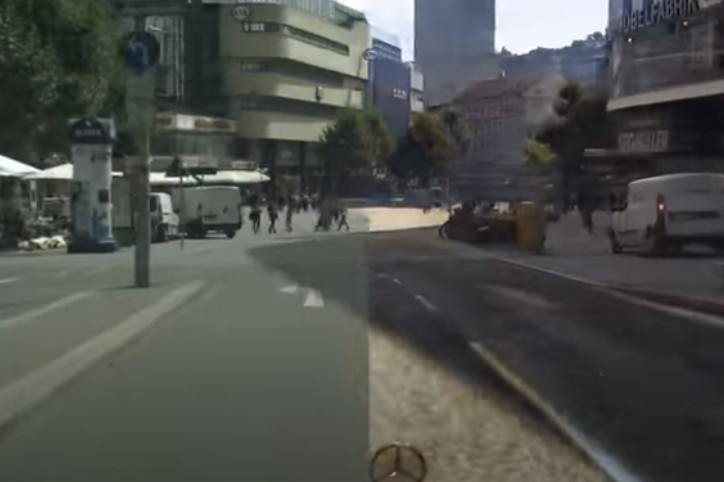
\includegraphics[width=7cm]{images/cyclegan-gta}}
		{\centering Image from \href{https://www.youtube.com/watch?v=lCR9sT9mbis&t=14s}{youtube}}
	\end{center}

\end{frame}


\begin{frame}
	\frametitle{GANs}
	\framesubtitle{Vanilla GANs}

	GANs are a general framework
	\begin{itemize}
		\item Generate samples indistinguishable from training data
		\item Many flavors exist
	\end{itemize}

	\bigskip

	Original GAN problem formulation
	\begin{itemize}
		\item Given samples $\vx$ (training data) from some distribution $P(\vx)$
		\item Learn to sample from this distribution
		\item In sense that $\cD$ cannot tell the difference
	\end{itemize}

\end{frame}


\begin{frame}
	\frametitle{GANs}
	\framesubtitle{Vanilla GANs}

	Got to make GAN stochastic %
	\begin{itemize}
		\item Add a source of randomness
		\item To enable new random generations
	\end{itemize}

	\bigskip

	To do so we replace input images to $\cG$ with $\vz$
	\begin{itemize}
		\item Fixed-size random vector, e.g.~$\vz\sim[-1,1]^{20}$ %
		\item Called \emph{latent vector}
	\end{itemize}

\end{frame}

\begin{frame}[fragile]
	\frametitle{GANs}
	\framesubtitle{Vanilla GANs}

	Changes to $\cG$
	\begin{itemize}
		\item Remove the encoder
		\item Instead map $\vz$ to suitable 3D tensor
	\end{itemize}

	\medskip

	\begin{verbatim}
def generator(nz):
  return nn.Sequential(
    nn.Linear(nz, 64 * 8 * 8),
    nn.ReLU(inplace=True),
    nn.Unflatten(1, (64, 8, 8)),
    ...  # rest of generator
  )
\end{verbatim}

\end{frame}


\begin{frame}
	\frametitle{GANs}
	\framesubtitle{Vanilla GANs}

	Resulting architecture
	\begin{itemize}
		\item Training works like before (image restoration)
	\end{itemize}

	\medskip

	\begin{center}
		\copyrightbox[b]
		{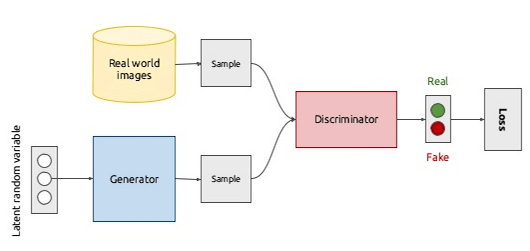
\includegraphics[width=7.5cm]{images/gan}}
		{\centering Image from sigmoidal.io}
	\end{center}

\end{frame}


\begin{frame}
	\frametitle{GANs}
	\framesubtitle{Vanilla GANs}

	Training such GANs can be a pain (unable to pre-train)
	\begin{itemize}
		\item Can fail for many reasons
	\end{itemize}

	\bigskip

	Two common issues
	\begin{itemize}
		\item $\cG$ cannot fool $\cD$ (vanishing gradients)
		\item $\cG$ generates similar outputs regardless of $\vz$ (\emph{mode collapse}) %
	\end{itemize}

	\bigskip

	Loss curves help identifying problems
	\begin{itemize}
		\item Loss on $\cD$ should never approach $0$
		\item Oscillations are bad
	\end{itemize}

\end{frame}


\begin{frame}
	\frametitle{GANs}
	\framesubtitle{Vanilla GANs}

	\begin{center}
		\copyrightbox[b]
		{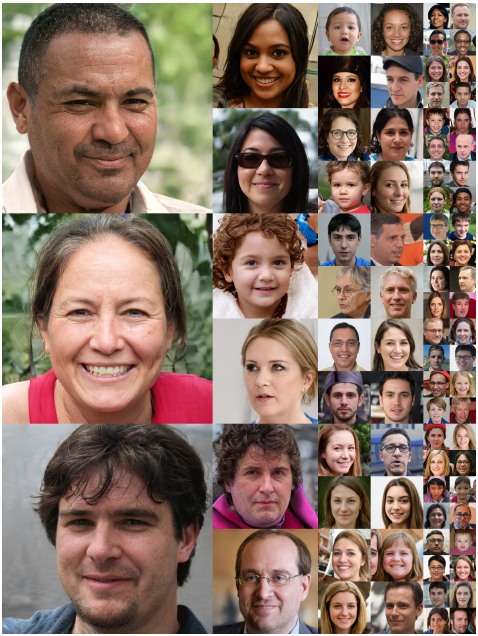
\includegraphics[width=4cm]{images/style-gan-faces}\hspace{0.5cm}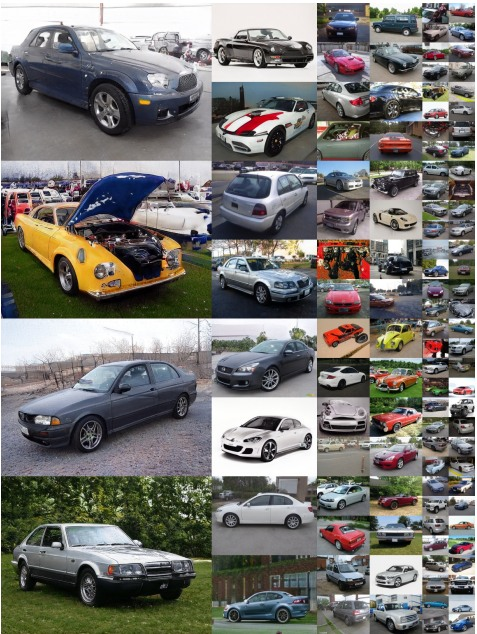
\includegraphics[width=4cm]{images/style-gan-cars}}
		{\centering Image from [3]}
	\end{center}

\end{frame}


\begin{frame}
	\frametitle{GANs}
	\framesubtitle{Conditional GANs}

	No intuitive way to control what $\cG$ should generate

	\bigskip

	If we train on CIFAR-10 for example
	\begin{itemize}
		\item Generated images will be of $10$ classes
		\item But we might want to e.g.~generate only car images
	\end{itemize}

	\bigskip

	\emph{Conditional GANs} overcome this limitation

\end{frame}


\begin{frame}
	\frametitle{GANs}
	\framesubtitle{Conditional GANs}

	Accomplished by adding another input $\vy$ to $\cG$ and $\cD$
	\begin{itemize}
		\item Where $\vy$ is what we want to condition on (e.g.~class label)
		\item Causing $\cG$ to learn to sample from $\Pr(\vx|\vy)$ %
	\end{itemize}

	\bigskip

	To generate random images of specific kind
	\begin{itemize}
		\item Choose $\vy$ accordingly (e.g.~desired class)
		\item Vary $\vz$ to generate different samples
	\end{itemize}

\end{frame}


\begin{frame}
	\frametitle{GANs}
	\framesubtitle{Conditional GANs}

	\begin{center}
		\copyrightbox[b]
		{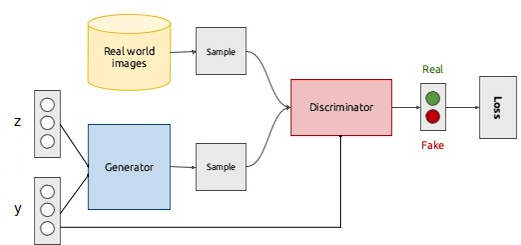
\includegraphics[width=9cm]{images/cgan}}
		{\centering Image adapted from sigmoidal.io}
	\end{center}

\end{frame}



\begin{frame}
	\frametitle{GANs}
	\framesubtitle{Conditional GANs}

	Many ways to define and incorporate $\vy$

	\bigskip

	Standard method for integer labels is an \emph{embedding}
	\begin{itemize}
		\item Learnable function $e:\{0,1,\dots,m-1\}\mapsto\RR^n$
		\item Maps positive numbers to fixed-size vectors
		\item $n$ is a hyperparameter
	\end{itemize}

	\bigskip

	\emph{Embedding layers} (e.g.~\texttt{torch.nn.Embedding})
	\begin{itemize}
		\item Have $m\times n$ parameters (initialized randomly)
		\item One learned vector of size $n$ per scalar input value (e.g.~class)
	\end{itemize}

\end{frame}


\begin{frame}
	\frametitle{GANs}
	\framesubtitle{Conditional GANs}

	Can set $n$ freely

	\bigskip

	In our context we set $n=H_0\cdot W_0$
	\begin{itemize}
		\item $H_0\times W_0$ is initial tensor height/width in $\cG$/$\cD$
		\item Allows us to then reshape to $1\times H_0\times W_0$
		\item Can then concatenate information as new channel
		\item To combine image and e.g.~class information in single tensor
	\end{itemize}

\end{frame}


\begin{frame}
	\frametitle{GANs}
	\framesubtitle{Conditional GANs}

	Class-conditional images generated by [4]

	\bigskip

	\begin{center}
		\copyrightbox[b]
		{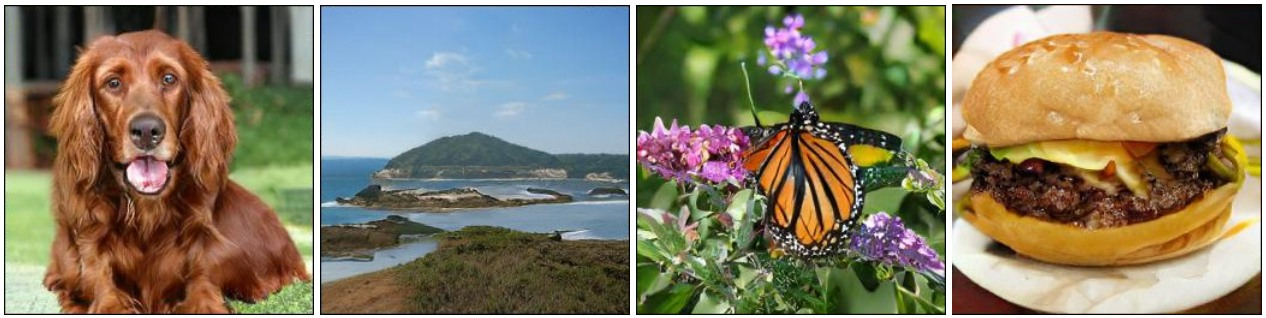
\includegraphics[width=10cm]{images/lsgan}}
		{\centering Image from [4]}
	\end{center}

\end{frame}


{
\setbeamertemplate{footline}{}
\begin{frame}

	\begin{tikzpicture}[remember picture,overlay]
		\fill[white] (current page.north west) rectangle (current page.south east);
	\end{tikzpicture}

	\begin{center}
		\textcolor[rgb]{0.9,0.9,0.9}{blank page}
	\end{center}

\end{frame}
}


\begin{frame}
	\frametitle{Transformers}

	We have focused on convolutional neural networks
	\begin{itemize}
		\item Dominating deep learning architecture for vision
	\end{itemize}

	\bigskip

	\emph{Transformers} are a new, strong competitor
	\begin{itemize}
		\item Originally proposed for \emph{natural language processing} (\emph{NLP}) [5]
		\item Recently adapted for vision (\emph{vision transformers}) (\emph{ViT}) [6]
	\end{itemize}

\end{frame}


\begin{frame}
	\frametitle{Transformers}
	\framesubtitle{Motivation}

	Recall inductive biases we derived for convnets
	\begin{itemize}
		\item Local connectivity
		\item Parameter sharing within feature maps
	\end{itemize}

	\bigskip

	These are solid inductive biases
	\begin{itemize}
		\item Sensible given how images are formed
		\item Significant reduction in parameters, computations over MLPs
		\item Enabling robust training of deep neural networks
	\end{itemize}

\end{frame}


\begin{frame}
	\frametitle{Transformers}
	\framesubtitle{Motivation}

	The are still biases though
	\begin{itemize}
		\item Likely not (always) optimal
		\item Particularly with respect to slowly increasing receptive field
	\end{itemize}

	\bigskip

	Transformers are more general
	\begin{itemize}
		\item Weaker task-specific inductive biases %
		\item General architecture with exceptional performance
	\end{itemize}

\end{frame}


\begin{frame}
	\frametitle{Transformers}
	\framesubtitle{Input}

	Transformers operate on \emph{sets} of vectors $\{\vt_1,\dots,\vt_S\}$
	\begin{itemize}
		\item Each vector $\vt_s\in\RR^T$ is called a \emph{token} %
		\item Token ordering must be encoded in $\vt_s$ (if relevant)
	\end{itemize}

	\bigskip

	The operation that characterizes transformers is \emph{attention}
	\begin{itemize}
		\item Compare all tokens to each other (details later)
		\item Time and memory complexity is $\approx\mathcal{O}(S^2)$ %
		\item Can become a limiting factor quickly as $S$ increases
	\end{itemize}

\end{frame}


\begin{frame}
	\frametitle{Transformers}
	\framesubtitle{Input}

	Got to convert input images accordingly
	\begin{itemize}
		\item Cannot just represent pixels as tokens ($S$ too big)
	\end{itemize}

	\bigskip

	ViTs split images into $S$ fixed-size patches (e.g.~$16\times16$) %
	\begin{itemize}
		\item Can be implemented using a conv layer with stride $k$ %
	\end{itemize}

	\medskip

	\begin{center}
		\copyrightbox[b]
		{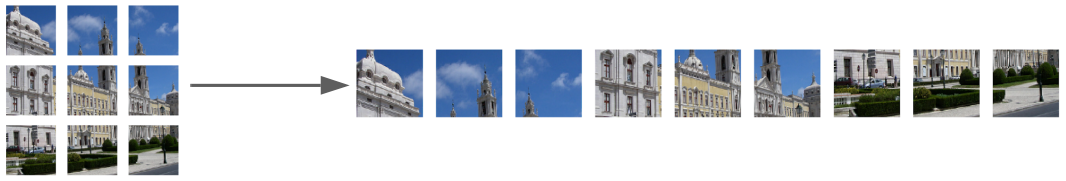
\includegraphics[width=9cm]{images/image-patches}}
		{\centering Image adapted from [6]}
	\end{center}

\end{frame}


\begin{frame}
	\frametitle{Transformers}
	\framesubtitle{Input}

	Patches are then flattened to vectors $\vv_s$ (size e.g.~$16\cdot16\cdot3$) %
	\begin{itemize}
		\item Original ViT [3] maps these to tokens via $\vt_s=\vv_s\vW$
		\item Learned weight matrix $\vW\in\RR^{\dim(\vt_s)\times T}$ (linear layer) %
	\end{itemize}

	\medskip

	\begin{center}
		\copyrightbox[b]
		{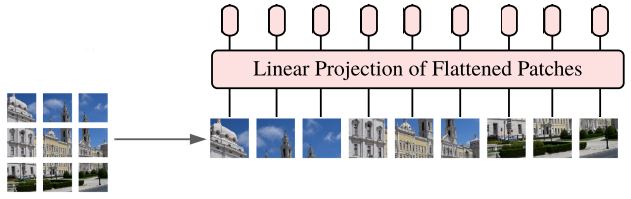
\includegraphics[width=9cm]{images/vit-input-tokens}}
		{\centering Image adapted from [6]}
	\end{center}

\end{frame}


\begin{frame}
	\frametitle{Transformers}
	\framesubtitle{Input}

	Patch location is certainly important (spatial information)
	\begin{itemize}
		\item Recall that we must encode this in $\vt_s$
		\item ViT [6] uses an embedding layer %
	\end{itemize}

	\medskip

	\begin{center}
		\copyrightbox[b]
		{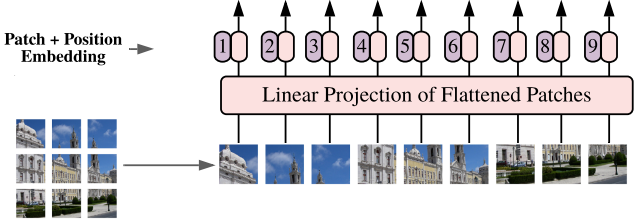
\includegraphics[width=9cm]{images/vit-positional}}
		{\centering Image adapted from [6]}
	\end{center}

\end{frame}


\begin{frame}
	\frametitle{Transformers}
	\framesubtitle{For Image Classification}

	Transformers map input tokens to output tokens
	\begin{itemize}
		\item Add a \emph{dummy token} (\emph{class embedding}) %
		\item Corresponding output token is input to classifier
	\end{itemize}

	\medskip

	\begin{center}
		\copyrightbox[b]
		{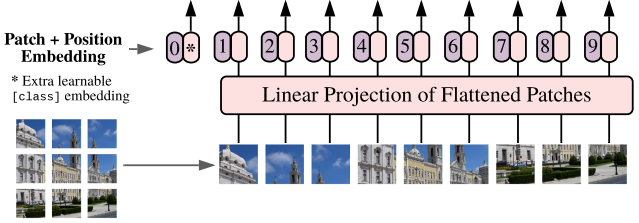
\includegraphics[width=9cm]{images/vit-positional-class}}
		{\centering Image adapted from [6]}
	\end{center}

\end{frame}


\begin{frame}
	\frametitle{Transformers}
	\framesubtitle{For Image Classification}

	\begin{center}
		\copyrightbox[b]
		{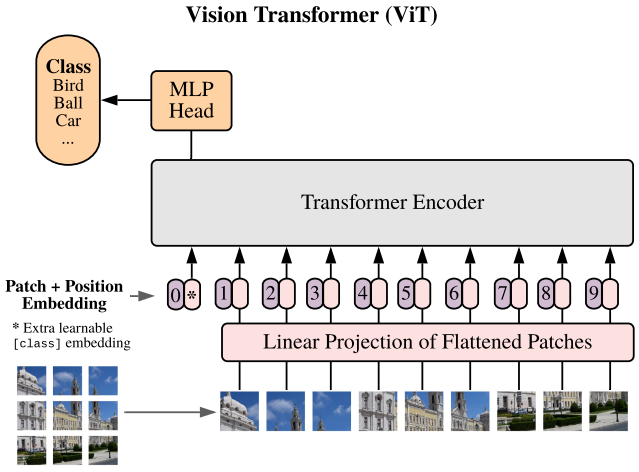
\includegraphics[width=8cm]{images/vit}}
		{\centering Image from [6]}
	\end{center}

\end{frame}


\begin{frame}
	\frametitle{Transformers}
	\framesubtitle{Transformer Encoder}

	\begin{columns}
		\column{0.75\linewidth}

		\emph{Transformer encoder} consists of $L$ sub-networks

		\bigskip

		Each network has identical architecture
		\begin{itemize}
			\item Input: $S\times T$ matrix of input tokens  %
			\item Output: $S\times T$ matrix of output tokens
			\item Skip-connections like ResNet
		\end{itemize}

		\column{0.25\linewidth}

		\begin{center}
			\copyrightbox[b]
			{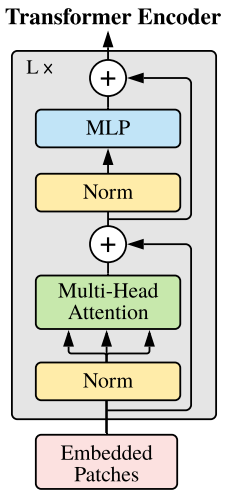
\includegraphics[width=2.5cm]{images/vit-encoder}}
			{\centering Image from [6]}
		\end{center}

	\end{columns}

\end{frame}


\begin{frame}
	\frametitle{Transformers}
	\framesubtitle{Transformer Encoder -- Normalization}

	\begin{columns}
		\column{0.75\linewidth}

		Normalization layers (yellow)
		\begin{itemize}
			\item Normalize individual rows ($\mu=0,\sigma=1$)
			\item Using Layer normalization
			\item To keep signals well-behaved as usual
		\end{itemize}

		\column{0.25\linewidth}

		\begin{center}
			\copyrightbox[b]
			{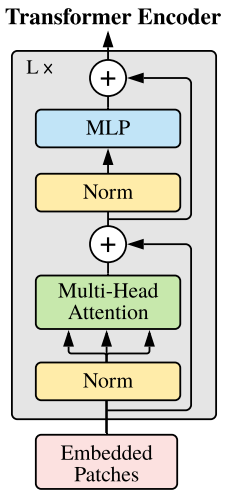
\includegraphics[width=2.5cm]{images/vit-encoder}}
			{\centering Image from [6]}
		\end{center}

	\end{columns}

\end{frame}


\begin{frame}[fragile]
	\frametitle{Transformers}
	\framesubtitle{Transformer Encoder -- MLP}

	\begin{columns}
		\column{0.75\linewidth}

		\emph{Gaussian Error Linear Unit} (\emph{GELU}) activation %
		\begin{itemize}
			\item Similar to ReLU
			\item Non-zero gradient for negative inputs %
		\end{itemize}

		\smallskip

		\begin{verbatim}
nn.Sequential(
    nn.Linear(dim, hidden_dim),
    nn.GELU(),
    nn.Dropout(dropout),
    nn.Linear(hidden_dim, dim),
    nn.Dropout(dropout)
)
\end{verbatim}

		\column{0.25\linewidth}

		\begin{center}
			\copyrightbox[b]
			{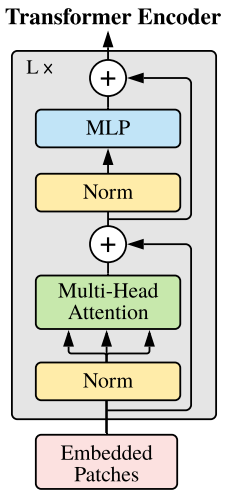
\includegraphics[width=2.5cm]{images/vit-encoder}}
			{\centering Image from [6]}
		\end{center}

	\end{columns}

\end{frame}


\begin{frame}
	\frametitle{Transformers}
	\framesubtitle{Transformer Encoder -- Multi-Head Attention}

	\begin{columns}
		\column{0.75\linewidth}

		Consists of $h$ independent attention layers

		\smallskip

		\begin{center}
			\copyrightbox[b]
			{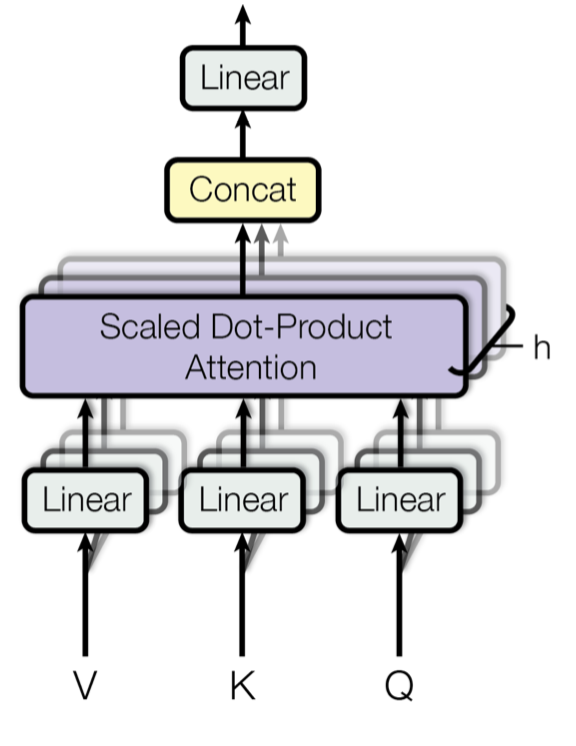
\includegraphics[width=4cm]{images/multi-head-attention}}
			{\centering Image from [5]}
		\end{center}

		\column{0.25\linewidth}

		\begin{center}
			\copyrightbox[b]
			{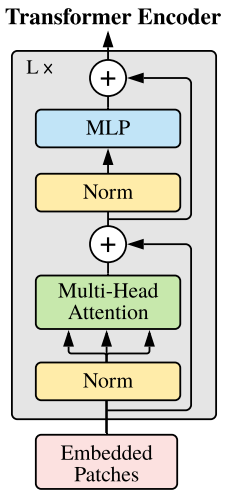
\includegraphics[width=2.5cm]{images/vit-encoder}}
			{\centering Image from [6]}
		\end{center}

	\end{columns}

\end{frame}


\begin{frame}
	\frametitle{Transformers}
	\framesubtitle{Transformer Encoder -- Attention}


	\begin{columns}
		\column{0.75\linewidth}

		$Q,K,V$ are $S\times H$ matrices
		\begin{itemize}
			\item Different learned linear projections of input
			\item $H$ is a hyperparameter
		\end{itemize}

		\bigskip

		\emph{Attention} is defined as
		\[
			\text{Attention}(Q,K,V)=\text{softmax}\left(\frac{Q\,K^T}{\sqrt{H}}\right)V %
		\]

		\column{0.25\linewidth}

		\begin{center}
			\copyrightbox[b]
			{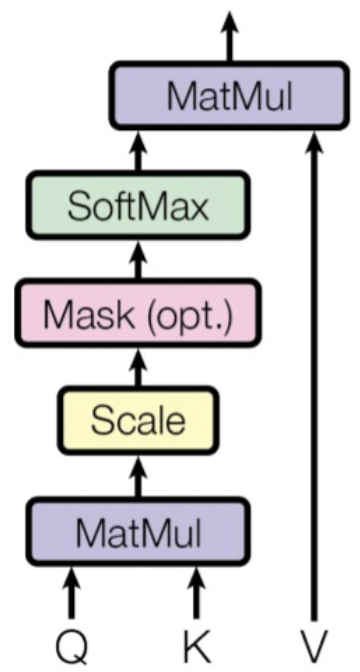
\includegraphics[width=2.5cm]{images/attention}}
			{\centering Image from [5]}
		\end{center}

	\end{columns}

\end{frame}


\begin{frame}
	\frametitle{Transformers}
	\framesubtitle{Transformer Encoder -- Attention}

	\begin{columns}
		\column{0.75\linewidth}

		$Q\,K^T$ is equal to dot products
		\begin{itemize}
			\item Between $S$ vectors in $Q$ and $S$ vectors in $K$
			\item Output has size $S\times S$ %
		\end{itemize}

		\bigskip

		Dot product encodes similarity between vectors
		\begin{itemize}
			\item Operation above computes similarity scores
		\end{itemize}

		\bigskip

		Softmax normalizes these scores to $[0,1]$

		\column{0.25\linewidth}

		\begin{center}
			\copyrightbox[b]
			{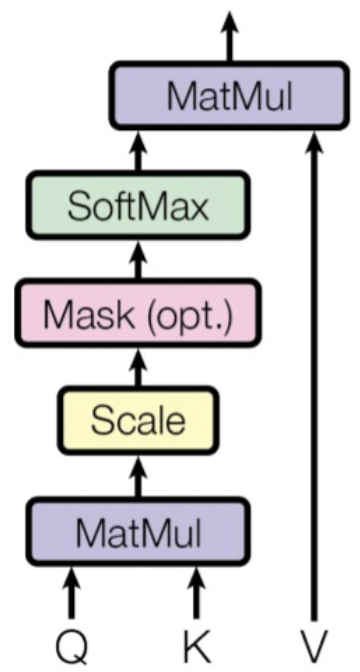
\includegraphics[width=2.5cm]{images/attention}}
			{\centering Image from [5]}
		\end{center}

	\end{columns}

\end{frame}


\begin{frame}
	\frametitle{Transformers}
	\framesubtitle{Transformer Encoder -- Attention}

	\begin{columns}
		\column{0.75\linewidth}

		Dot product $\text{softmax}(\cdot)\,V$
		\begin{itemize}
			\item Causes vectors of $V$ to be suppressed
			\item If similarity score between $Q$ and $K$ was small
		\end{itemize}

		\bigskip

		Encodes which vectors rest should focus on
		\begin{itemize}
			\item Vectors correspond to tokens / patches
		\end{itemize}

		\column{0.25\linewidth}

		\begin{center}
			\copyrightbox[b]
			{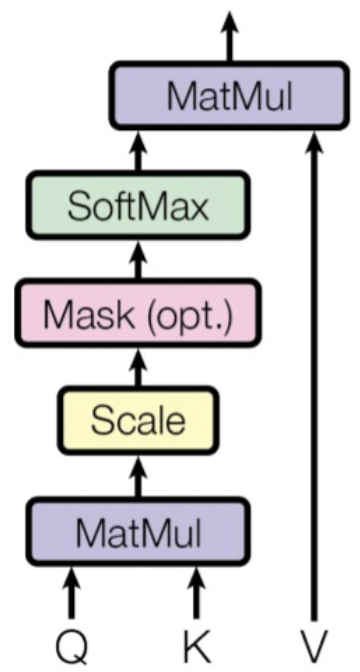
\includegraphics[width=2.5cm]{images/attention}}
			{\centering Image from [5]}
		\end{center}

	\end{columns}

\end{frame}


\begin{frame}
	\frametitle{Transformers}
	\framesubtitle{Training}

	Training is done as usual
	\begin{itemize}
		\item Backpropagation to compute $\nabla L(\bth)$
		\item Iterative optimization (Adam is popular)
	\end{itemize}

\end{frame}


\begin{frame}
	\frametitle{Transformers}
	\framesubtitle{Versus Conv Nets}

	Transformers have a global receptive field
	\begin{itemize}
		\item Every layer sees everything (in contrast to conv nets)
	\end{itemize}

	\medskip

	\begin{center}
		\copyrightbox[b]
		{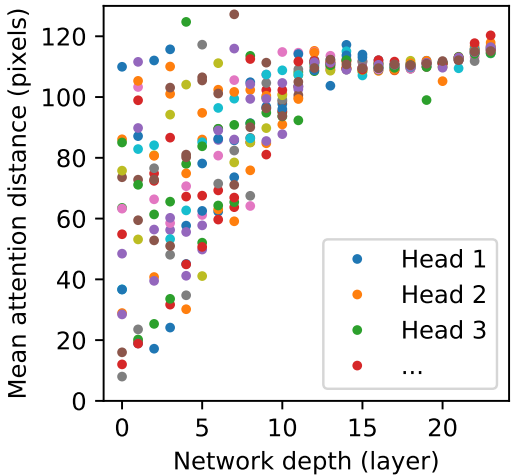
\includegraphics[width=4.5cm]{images/attention-distance}}
		{\centering Image adapted from [6]}
	\end{center}

\end{frame}


\begin{frame}
	\frametitle{Transformers}
	\framesubtitle{Versus Conv Nets}

	Transformers might scale better to huge datasets
	\begin{itemize}
		\item Many millions of images
	\end{itemize}

	\bigskip

	Transformers currently top many vision task leaderboards
	\begin{itemize}
		\item Advantage over modern conv nets is usually small though
		\item Not necessarily because of inherently better architecture
	\end{itemize}

	\bigskip

	No clear winner in terms of training and inference times
	\begin{itemize}
		\item Varies a lot depending on particular architectures
	\end{itemize}

\end{frame}


\begin{frame}
	\frametitle{Transformers}
	\framesubtitle{Remarks}

	Transformers are all the rage right now
	\begin{itemize}
		\item Fast progress
	\end{itemize}

	\bigskip
	Transformers are the foundation of \emph{large language models} (\emph{LLMs})
	\begin{itemize}
		\item Such as GPT-4 (ChatGPT), PaLM (Bard)
	\end{itemize}

\end{frame}


\renewcommand\emph[1]{\oldemph{#1}}

\begin{frame}
	\frametitle{Bibliography}

	[1] Isola et al.~\href{https://arxiv.org/abs/1611.07004}{Pix2Pix}.~2016\\\medskip
	[2] Zhu et al.~\href{https://arxiv.org/abs/1703.10593}{CycleGAN}.~2017\\\medskip
	[3] Karras et  al.~\href{https://arxiv.org/abs/1812.04948}{StyleGAN}.~2018\\\medskip
	[4] Brock et al.~\href{https://arxiv.org/abs/1809.11096}{Large-Scale GAN}.~2019\\\medskip
	[5] Vaswani et al.~\href{https://arxiv.org/abs/1706.03762v5}{Transformers}.~2017\\\medskip
	[6] Dosovitskiy at al.~\href{https://arxiv.org/abs/2010.11929}{Vision Transformers}.~2020\\\medskip

\end{frame}


\end{document}
